\documentclass[a4paper, 10pt]{article}

%\usepackage{showframe}
\usepackage{geometry}
\usepackage{xcolor}
\usepackage[absolute]{textpos}
\usepackage[most]{tcolorbox}
\usepackage{lipsum}
\usepackage{graphicx}
\usepackage{duckuments}
\usepackage{fontawesome5}
\usepackage{setspace}
\usepackage{hyperref}
\usepackage{booktabs}
\usepackage{svg}
\usepackage{import}
\usepackage{enumitem}
\usepackage[style=authoryear]{biblatex}


\addbibresource{publications.bib}
\nocite{*}

\TPGrid[0mm,0mm]{10}{10}

\tcbuselibrary{raster}
\geometry{left=1.0cm, right=0.5cm, top=1.0cm, bottom=1.0cm}

\definecolor{sidebar}{RGB}{233,233,233}
\definecolor{textgray}{RGB}{73,73,73}
\textblockcolour{sidebar}

\newcommand{\IconSize}{0.15}
\newcommand{\Icon}[3]{
    \begin{minipage}[c]{#1\textwidth}
        \vspace*{4pt}
        \includegraphics[width=#2\textwidth]{#3}
    \end{minipage}
}

\newcommand{\CVEntry}[3]{
    \begin{minipage}[t]{0.23\textwidth}
        \textbf{#1}
    \end{minipage}%
    \begin{minipage}[t]{0.76\textwidth}
        %\textbf{\large #2}\\
        \textbf{#2}\\
        #3
    \end{minipage}%
}

\newcommand{\CVSubEntry}[2]{
    \begin{minipage}[t]{0.23\textwidth}
        \vspace{3pt}
        \hspace{8pt}#1
    \end{minipage}%
    \begin{minipage}[t]{0.76\textwidth}
        \vspace{3pt}
        #2
    \end{minipage}%
}

\newlist{keyskills}{itemize}{3}
\setlist[keyskills,1]{label=\textbullet,leftmargin=6mm}

\begin{document}
\thispagestyle{empty}

\begin{tcbraster}[raster columns=7]
\begin{tcolorbox}[left=4pt, right=4pt, top=4pt, height=1.0\textheight, colback=sidebar, boxrule=0.5pt, arc=8pt, frame empty, raster multicolumn=2, nobeforeafter]
    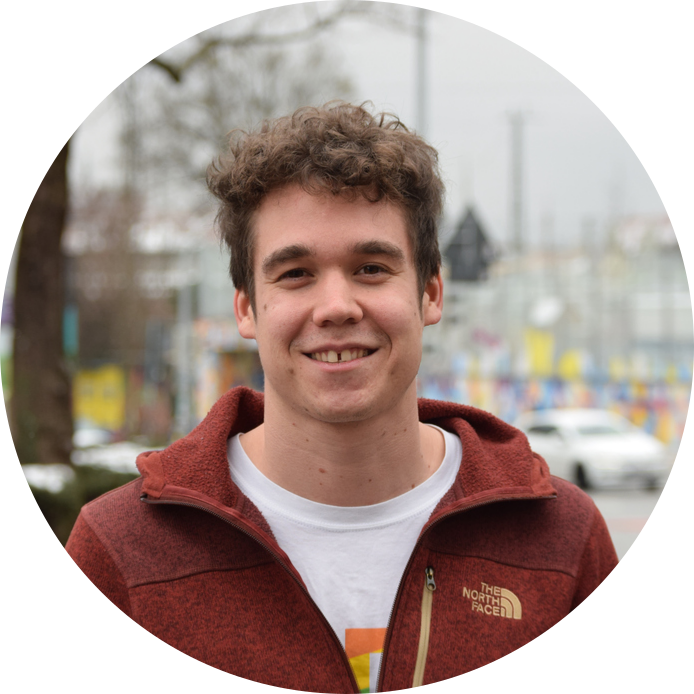
\includegraphics[width=1.0\linewidth]{./src/profile_pic_round.png}
    %\includegraphics[width=1.0\linewidth]{./src/profile_pic.png}
    %\includegraphics[width=1.0\linewidth]{./src/profile_pic_rounded.png}
    \begin{center}
        {\large \textbf{Timo Bachmann}} \\
    \end{center}

    \vspace{6mm}
    \begin{center}
        {\textbf{CONTACT}} \\
    \end{center}
    \small
    \begin{spacing}{1.325}
        \hspace*{10pt}\faIcon{globe-americas} \href{https://tfachmann.com}{tfachmann.com} \\
        \hspace*{10pt}\faIcon{envelope} \href{mailto:bachmanntj@gmail.com}{bachmanntj@gmail.com} \\
        \hspace*{10pt}\faIcon{github} \href{https://github.com/tfachmann}{tfachmann} \\
        \hspace*{10pt}\faIcon{phone} +49 175 8682972 \\
        \hspace*{10pt}\faIcon{home} 80337 Munich, Germany \\
        \hspace*{10pt}\faIcon{birthday-cake} April 12, 1998 \\
        \hspace*{10pt}\faIcon{flag} German, Swiss
    \end{spacing}
    \vspace{6mm}

    \begin{center}
        {\textbf{ABOUT ME}} \\
    \end{center}
    \begin{center}
        Passionate about making things work and learning new tools.
        Dives deep into nerdy topics of Linux, new programming languages and paradigms, software engineering and machine learning.
        Strong focus on writing readable, testable, paralellizable and safe source code.
        A terminal with Vim and tmux is all I need.
        Likes hiking and poetry.
    \end{center}

    \vspace{4mm}
    \begin{center}
        {\textbf{KEY SKILLS}} \\
    \end{center}

    \begin{keyskills}
        \item \textbf{Artificial Intelligence}\\ ML, data vis, optimization
        \item \textbf{Robotics}\\ 7-DoF LWRs, Ontologies
        \item \textbf{CI \& Deployment}\\ Conan, Docker, Jenkins
        \item \textbf{Linux \& Terminal}\\ Fast with linux, vim, tmux
        \item \textbf{Languages}\\ C{}\verb|++|, Python, Rust
    \end{keyskills}

    \vspace{8mm}
    \begin{center}
        {\textbf{LANGUAGES}} \\
    \end{center}
    \begin{center}
        \begin{tabular}[c]{rl}
            \textbf{German} & Native \\
            \textbf{English} & C2 \\
            \textbf{French} & B1 \\
        \end{tabular}
    \end{center}


\end{tcolorbox}
\begin{tcolorbox}[left=1cm, height=1.0\textheight, colback=white, raster multicolumn=5, boxrule=0pt, frame empty, nobeforeafter]
    \section*{Education}
    \CVEntry{2021 -- Now}{Technical University Munich (TUM)}{
        M.Sc.\ Robotics, Cognition, Intelligence\\
        Current grade: 1.9\\
    }
    \CVEntry{2017 -- 2020}{Cooperative State University Mannheim (DHBW)}{
        B.Sc.\ Information and Communication Technology\\
        German Aerospace Center (DLR)\\
        Final grade: 1.3\\
    }
    \CVEntry{2007 -- 2016}{Allgemeine Hochschulreife}{
        Alexander-von-Humboldt Gymnasium\\
        Final grade: 1.3\\
    }
    \vspace{5mm}
    \section*{Work Experience}
    \CVEntry{2017 -- Now}{German Aerospace Center (DLR)}{
        Department of Cognitive Robotics, Industrial Robotics
    }%
    \CVSubEntry{2020 -- Now}{
        Research Scientist and Engineer
        {
            \small\begin{spacing}{0.9}
            Kinematic workspace analysis, autonomous task execution and ontological representation of data in the industrial robotics domain.
            \end{spacing}%
            \vspace{2pt}
        }%
    }%
    \CVSubEntry{2017 -- 2020}{
        Working Student
        {
            \small\begin{spacing}{0.9}
            Joint dual study program with DHBW.
            \end{spacing}%
            \vspace{2pt}
        }
    }\\\\
    \CVEntry{2016 -- 2017}{Robert-Dyckerhoff Foundation, Thailand}{
        Volunteer -- Teaching English language\\
    }
    \vspace{5mm}
    \printbibliography[title=Publications]

    \vspace{5mm}
    \section*{Skills and Tools}
    \begin{tcbraster}[raster columns=2]
        \begin{tcolorbox}[colback=white, boxrule=0pt, frame empty, nobeforeafter]
            {\color{textgray} Core Programming Languages }\\
            \Icon{\IconSize}{1.15}{./src/cpp.pdf}
            \Icon{\IconSize}{1.1}{./src/python.pdf}
            \Icon{\IconSize}{1.3}{./src/rust.pdf}
            \\\\
            {\color{textgray} Deployment Tools }\\
            \Icon{\IconSize}{1.1}{./src/cmake.pdf}
            \Icon{\IconSize}{1.1}{./src/conan.pdf}
            \Icon{\IconSize}{1.3}{./src/docker.pdf}
            \Icon{\IconSize}{1.05}{./src/jenkins.pdf}
            \Icon{\IconSize}{1.1}{./src/artifactory.pdf}
            \\\\
            {\color{textgray} Other Tools }\\
            \Icon{\IconSize}{1.0}{./src/neovim.pdf}
            \hspace*{-6pt}
            \Icon{\IconSize}{1.25}{./src/github.pdf}
            \Icon{\IconSize}{1.1}{./src/javascript.pdf}
            \Icon{\IconSize}{1.1}{./src/webassembly.pdf}
            \begin{minipage}[c]{\IconSize\textwidth}
                \vspace*{4pt}
                \hspace*{-3.5pt}
                \LARGE \LaTeX
            \end{minipage}
        \end{tcolorbox}
    \end{tcbraster}
\end{tcolorbox}
\end{tcbraster}

\end{document}
